\documentclass[beamer,crop,tikz]{standalone}

\usepackage{formation}

\begin{document}
  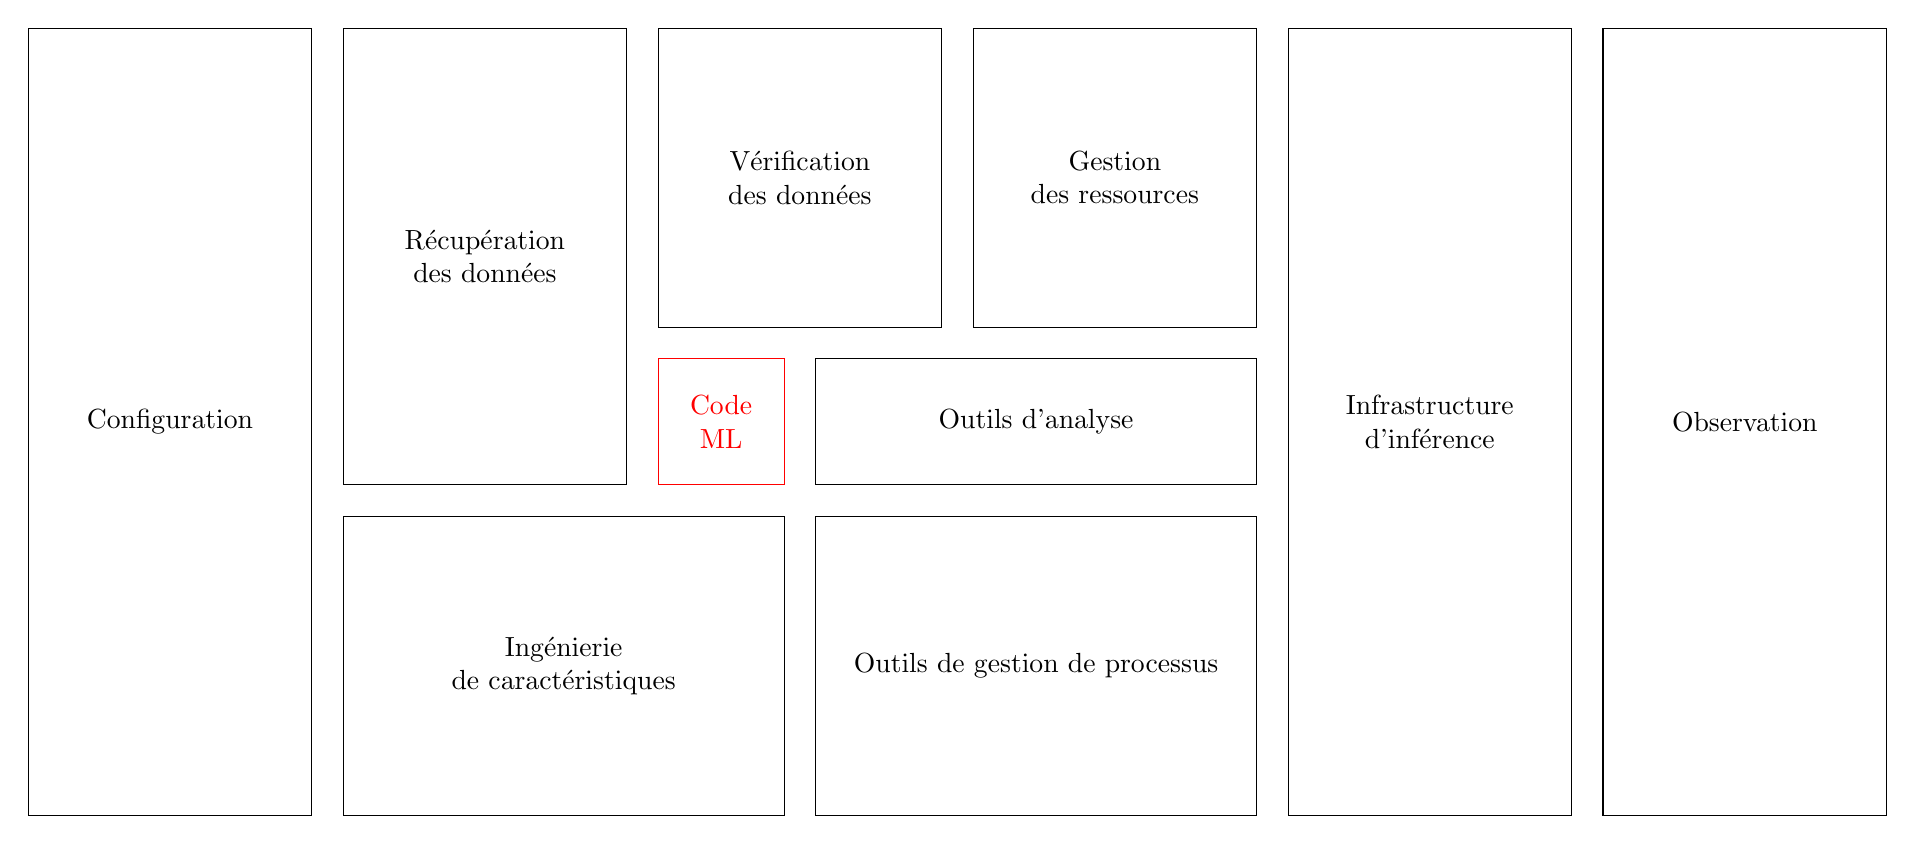
\begin{tikzpicture}
    \draw[align=center] (0.2, 0) rectangle (3.8, 10) node[midway] {Configuration};
    \draw[align=center] (4.2, 4.2) rectangle (7.8, 10) node[midway] {Récupération\\des données};
    \draw[align=center] (4.2, 0) rectangle (9.8, 3.8) node[midway] {Ingénierie\\de caractéristiques};
    \draw[align=center, color=red] (8.2, 4.2) rectangle (9.8, 5.8) node[midway] {Code\\ML};
    \draw[align=center] (8.2, 6.2) rectangle (11.8, 10) node[midway] {Vérification\\des données};
    \draw[align=center] (12.2, 6.2) rectangle (15.8, 10) node[midway] {Gestion\\des ressources};
    \draw[align=center] (10.2, 4.2) rectangle (15.8, 5.8) node[midway] {Outils d'analyse};
    \draw[align=center] (10.2, 0) rectangle (15.8, 3.8) node[midway] {Outils de gestion de processus};
    \draw[align=center] (16.2, 0) rectangle (19.8, 10) node[midway] {Infrastructure\\d'inférence};
    \draw[align=center] (20.2, 0) rectangle (23.8, 10) node[midway] {Observation};
  \end{tikzpicture}
\end{document}
